\chapter{Research Methodology}

\section{Research Design Overview}

This study employs a quantitative research approach to analyse network traffic patterns and develop machine learning models for malware detection. The research follows a systematic process comprising four main phases: (1) data acquisition and preparation, (2) exploratory data analysis, (3) model development and optimisation, and (4) performance evaluation. This methodology aligns with established practices in cybersecurity research, where empirical evidence from real-world data forms the foundation for developing detection systems.

Figure \ref{fig:methodology_overview} presents a visual overview of the research methodology, illustrating the flow from data collection to model evaluation.

\begin{figure}[ht]
    \centering
    \begin{tikzpicture}[
        node distance=2cm,
        phase/.style={rectangle, rounded corners, draw=black, fill=blue!10, minimum width=2.5cm, minimum height=1cm, align=center, font=\sffamily\bfseries},
        process/.style={rectangle, draw=black, fill=gray!5, minimum width=2.2cm, minimum height=0.7cm, align=center, font=\sffamily\small},
        arrow/.style={thick, ->, >=stealth},
    ]
    
    % Main phases (horizontal layout)
    \node[phase] (data) {1. Data};
    \node[phase, right=of data] (eda) {2. Analysis};
    \node[phase, right=of eda] (model) {3. Modeling};
    \node[phase, right=of model] (eval) {4. Evaluation};
    
    % Sub-processes below each phase
    \node[process, below=0.8cm of data] (clean) {Cleaning};
    \node[process, below=0.5cm of clean] (feat) {Engineering};
    
    \node[process, below=0.8cm of eda] (dist) {Distribution};
    \node[process, below=0.5cm of dist] (corr) {Correlation};
    
    \node[process, below=0.8cm of model] (select) {Feature Selection};
    \node[process, below=0.5cm of select] (train) {Training};
    
    \node[process, below=0.8cm of eval] (metrics) {Metrics};
    \node[process, below=0.5cm of metrics] (compare) {Comparison};
    
    % Connect main phases
    \draw[arrow] (data) -- (eda);
    \draw[arrow] (eda) -- (model);
    \draw[arrow] (model) -- (eval);
    
    % Connect sub-processes to their phases
    \draw[arrow] (data) -- (clean);
    \draw[arrow] (clean) -- (feat);
    
    \draw[arrow] (eda) -- (dist);
    \draw[arrow] (dist) -- (corr);
    
    \draw[arrow] (model) -- (select);
    \draw[arrow] (select) -- (train);
    
    \draw[arrow] (eval) -- (metrics);
    \draw[arrow] (metrics) -- (compare);
    
    % Feedback loop
    \draw[arrow] (eval.north) -- ++(0,0.5) -| (data.north);
    
    \end{tikzpicture}
    \caption{Research methodology workflow from data acquisition to evaluation}
    \label{fig:methodology_overview}
\end{figure}

The research design incorporates descriptive and inferential statistical methods to analyse the characteristics of network traffic and identify patterns associated with malicious activities. By combining exploratory visualisation techniques with machine learning algorithms, this approach enables both the discovery of underlying patterns in the data and the development of predictive models that can generalise to new unseen traffic. The following sections describe each component of the methodology in detail.

\section{Dataset Description}

\subsection{Dataset Source and Collection}

This research utilises the CTU-IoT-Malware dataset, collected by the Stratosphere Laboratory at the Czech Technical University (CTU). The dataset consists of network traffic captures from real IoT devices infected with malware, alongside benign traffic from the same network environment. These captures represent realistic attack scenarios rather than simulated environments, providing a more authentic basis for analysis. The dataset is publicly available and can be accessed at \url{https://www.stratosphereips.org/datasets-iot23} and kaggle \url{https://www.kaggle.com/datasets/agungpambudi/network-malware-detection-connection-analysis}. We are making use of the kaggle dataset for this research.

The dataset was collected using network monitoring equipment that recorded all traffic flows between monitored devices and external networks. Each connection was labelled according to known malicious IP addresses, domain names, and behaviour patterns identified by security researchers. The dataset includes multiple capture files representing different attack scenarios and device types.

For this research, we focus primarily on the connection log files (.conn files), which contain metadata about each network connection without the raw packet data, thus avoiding privacy concerns while still providing sufficient information for traffic analysis.

The analysed dataset contains more than one million labelled network connections with 23 features for each connection. Key features include:

\begin{table}[h]
\centering
\begin{tabular}{lp{0.6\textwidth}}
\hline
\textbf{Feature} & \textbf{Description} \\
\hline
Timestamp (ts) & Indicates the date and time when the connection occurred. \\
\hline
Source and Destination Information & Consists of the following fields: \\
 & \quad id.orig\_h: Source IP address \\
 & \quad id.orig\_p: Source port \\
 & \quad id.resp\_h: Destination IP address \\
 & \quad id.resp\_p: Destination port \\
\hline
Protocol (proto) & Specifies the network protocol used (e.g., TCP, UDP, or ICMP). \\
\hline
Connection state (conn\_state) & Flags that indicate the status of the connection, such as S0 (no response), SF (normal termination), or REJ (rejected). \\
\hline
Byte counts (orig\_bytes, resp\_bytes) & Represent the volume of data transferred from the source and destination, respectively. \\
\hline
Packet counts (orig\_pkts, resp\_pkts) & The number of packets sent from the source and to the destination, respectively. \\
\hline
Duration & The total time (in seconds) that the connection lasted. \\
\hline
Label & Classifies the connection as either "Malicious" or "Benign". \\
\hline
Detailed-label & Provides a specific attack type for malicious connections, offering more granular insight into the threat. \\
\hline
\end{tabular}
\caption{Dataset Features with Detailed Explanations}
\label{tab:dataset_features}
\end{table}

Initial analysis showed that the dataset contains approximately 53.5\% malicious connections and 46.5\% benign connections, providing a relatively balanced basis for classification tasks.

\section{Data Preprocessing}

The data cleaning process addressed several challenges in the raw dataset to ensure quality and consistency. Initial analysis revealed that missing values affected 79\% of records in certain columns, primarily in connections representing scanning activities where connections were attempted but not established.

We identified and resolved four main types of data quality issues:

\begin{enumerate}
    \item \textbf{Missing values}: For features like duration, orig\_bytes, and resp\_bytes, we applied domain-specific imputation strategies. Byte and packet counts were imputed with zeros (representing no data transfer), while duration values were imputed using protocol-connection state conditional medians. Binary indicators tracked missingness patterns, which proved informative for classification.
    
    \item \textbf{Type conversion}: Timestamps were converted to date-time objects, categorical variables (protocol, connection state) were encoded using appropriate schemes, and string representations were standardised throughout the dataset.
    
    \item \textbf{Outlier handling}: For numeric features (duration, byte counts, packet counts), we applied the log transformation ($x' = \log(x + 1)$) to address the heavily biased distributions common in network traffic data. Statistical outliers were then identified using the interquartile range (IQR) method, with extreme values capped at $Q_3 + 1.5 \times \text{IQR}$. Z-score normalisation was applied for values where $|z| > 3$.
    
    \item \textbf{Label standardisation}: Inconsistent labels were cleaned, detailed labels were extracted from compound fields, and consistency of binary classification was ensured throughout.
\end{enumerate}

The mathematical formulation of the data cleaning process is as follows:

\begin{itemize}
    \item For missing byte and packet counts:
    \begin{equation}
        x_{i,j} = 
        \begin{cases}
            x_{i,j} & \text{if } x_{i,j} \text{ exists} \\
            0 & \text{if } x_{i,j} \text{ is missing}
        \end{cases}
    \end{equation}
    where $x_{i,j}$ represents feature $j$ for connection $i$.
    
    \item For duration values:
    \begin{equation}
        \text{duration}_{i} = 
        \begin{cases}
            \text{duration}_{i} & \text{if exists} \\
            \text{median}(\text{duration} \mid \text{proto}=p_i, \text{conn\_state}=c_i) & \text{otherwise}
        \end{cases}
    \end{equation}
    where $p_i$ and $c_i$ are the protocol and connection state of connection $i$.
    
    \item For outlier identification:
    \begin{equation}
        \text{outlier}(x_i) = 
        \begin{cases}
            \text{True} & \text{if } x_i < Q_1 - 1.5 \times \text{IQR} \text{ or } x_i > Q_3 + 1.5 \times \text{IQR} \\
            \text{False} & \text{otherwise}
        \end{cases}
    \end{equation}
    where $Q_1$ and $Q_3$ are the first and third quartiles, and $\text{IQR} = Q_3 - Q_1$.
    
    \item For log transformation:
    \begin{equation}
        x'_i = \log(x_i + 1)
    \end{equation}
    The addition of 1 prevents undefined values when $x_i = 0$, which is common for scanning connections.
\end{itemize}

These preprocessing steps resulted in a consistent and analysis-ready dataset that preserved the meaningful characteristics of network traffic while addressing data quality issues.

During the exploratory data analysis phase, various visualisation and statistical techniques were applied to understand the characteristics of the dataset. The distribution analysis of key features was performed using histograms and kernel density estimation to reveal the spread and central tendencies within the data. In parallel, a correlation analysis between numeric features was performed to identify underlying relationships that could influence the performance of the model.

The analysis also included an examination of temporal patterns to detect time-based attack behaviours, along with an assessment of protocol and connection state variations across different traffic classes. Furthermore, principal component analysis (PCA) was used for dimensionality reduction, which helped in assessing the relative importance of various features. These insights collectively informed the subsequent processes of feature selection and model development.

\section{Feature Engineering}

Based on domain knowledge and exploratory analysis, we derived additional features to enhance the malware detection capability of our models. These engineered features fall into three main categories: temporal features, traffic characteristics, and behavioural indicators. The following describe the derived features in detail.

\subsubsection{Temporal Features}

Temporal patterns often reveal coordinated attacks and scanning behaviours. We extracted the following time-based features:

\begin{itemize}
    \item \textbf{Hour of day}: $\text{hour}_i = \text{hour}(\text{timestamp}_i) \in \{0,1,\ldots,23\}$
    
    \item \textbf{Day of week}: $\text{day\_of\_week}_i = \text{weekday}(\text{timestamp}_i) \in \{0,1,\ldots,6\}$
    
    \item \textbf{Weekend indicator}: $\text{is\_weekend}_i = \mathbb{1}[\text{day\_of\_week}_i \in \{5,6\}]$, where $\mathbb{1}[\cdot]$ is the indicator function
\end{itemize}

\subsubsection{Traffic Volume Features}

Traffic volume characteristics help distinguish scanning activities from legitimate data transfers:

\begin{itemize}
    \item \textbf{Total bytes}: $\text{total\_bytes}_i = \text{orig\_bytes}_i + \text{resp\_bytes}_i$
    
    \item \textbf{Total packets}: $\text{total\_pkts}_i = \text{orig\_pkts}_i + \text{resp\_pkts}_i$
    
    \item \textbf{Bytes per packet ratio}: To capture the efficiency of data transfer, we calculated:
    \begin{equation}
        \text{orig\_bytes\_per\_pkt}_i = \frac{\text{orig\_bytes}_i}{\text{orig\_pkts}_i + \epsilon}
    \end{equation}
    \begin{equation}
        \text{resp\_bytes\_per\_pkt}_i = \frac{\text{resp\_bytes}_i}{\text{resp\_pkts}_i + \epsilon}
    \end{equation}
    where $\epsilon = 1$ to avoid division by zero when no packets were sent.
    
    \item \textbf{Bytes ratio}: To capture the directionality of traffic, we calculated:
    \begin{equation}
        \text{bytes\_ratio}_i = \frac{\text{orig\_bytes}_i}{\text{resp\_bytes}_i + \epsilon}
    \end{equation}
    
    \item \textbf{Packets ratio}: Similarly, for packet counts:
    \begin{equation}
        \text{pkts\_ratio}_i = \frac{\text{orig\_pkts}_i}{\text{resp\_pkts}_i + \epsilon}
    \end{equation}
\end{itemize}

The final preprocessed dataset contained 27 features, including 23 original features and 4 engineered features. This comprehensive feature set provided a rich representation of network traffic patterns for machine learning models.

\section{Machine Learning Approach}

Based on the findings of the exploratory analysis, we selected three machine learning algorithms for the malware detection task, each with distinct strengths and theoretical foundations. The selected algorithms are the following:

\begin{itemize}
    \item Random Forest
    \item Support Vector Machine
    \item XGBoost
\end{itemize}

In addition, we implemented a deep learning approach using a feed-forward neural network. The following subsections describe the mathematical formulations and theoretical underpinnings of each algorithm. The models were implemented using the Scikit-learn library for traditional machine learning algorithms and PyTorch for the deep learning model. The models were trained on a balanced subset of the dataset, ensuring that both benign and malicious classes were equally represented.

\subsection{Random Forest Classification}

Random Forest is an ensemble learning method that constructs multiple decision trees during training and outputs the class that is the mode of the individual trees' predictions. For a given input vector $\mathbf{x}$, the Random Forest model predicts:

\begin{equation}
\hat{y}(\mathbf{x}) = \frac{1}{B} \sum_{b=1}^{B} h_b(\mathbf{x}, \Theta_b)
\end{equation}

where $h_b$ is the $b^{th}$ decision tree trained with a random subset of features determined by $\Theta_b$, and $B$ is the total number of trees in the forest. 

Each decision tree partitions the feature space recursively based on the Gini impurity measure, which for a node $t$ is defined as:

\begin{equation}
G(t) = 1 - \sum_{i=1}^{C} p_i^2
\end{equation}

where $C$ is the number of classes (2 in our case) and $p_i$ is the proportion of class samples $i$ in node $t$. The feature and threshold that minimise the weighted sum of child-node impurities are selected for each split.

\subsection{Support Vector Machine Classification}

Support Vector Machines find the hyperplane that maximally separates the classes in feature space. For non-linearly separable data, the kernel trick is applied to transform the input space into a higher-dimensional feature space where linear separation is possible. The SVM decision function is as follows.

\begin{equation}
f(\mathbf{x}) = \text{sign}\left(\sum_{i=1}^{N} \alpha_i y_i K(\mathbf{x}_i, \mathbf{x}) + b\right)
\end{equation}

where $\alpha_i$ are the Lagrange multipliers obtained by solving the dual optimisation problem:

\begin{equation}
\begin{aligned}
\text{maximize } & \sum_{i=1}^{N} \alpha_i - \frac{1}{2} \sum_{i=1}^{N} \sum_{j=1}^{N} \alpha_i \alpha_j y_i y_j K(\mathbf{x}_i, \mathbf{x}_j) \\
\text{subject to } & 0 \leq \alpha_i \leq C, \quad i = 1, 2, ..., N \\
& \sum_{i=1}^{N} \alpha_i y_i = 0
\end{aligned}
\end{equation}

where $C$ is the regularisation parameter that controls the trade-off between the maximisation of the margin and the classification error, and $K(\mathbf{x}_i, \mathbf{x}_j)$ is the kernel function. We used the radial basis function (RBF) kernel:

\begin{equation}
K(\mathbf{x}_i, \mathbf{x}_j) = \exp\left(-\gamma \|\mathbf{x}_i - \mathbf{x}_j\|^2\right)
\end{equation}

where $\gamma$ controls the influence range of each support vector.

\subsection{XGBoost Classification}

XGBoost (eXtreme Gradient Boosting) is an optimised implementation of gradient boosting that sequentially adds decision trees to correct errors made by existing trees. The model is built by minimising the objective function:

\begin{equation}
\mathcal{L}(\phi) = \sum_{i=1}^{N} l(y_i, \hat{y}_i) + \sum_{k=1}^{K} \Omega(f_k)
\end{equation}

where $l$ is the loss function (logistic loss for binary classification), $\hat{y}_i$ is the predicted probability, and $\Omega$ is the regularisation term defined as:

\begin{equation}
\Omega(f) = \gamma T + \frac{1}{2}\lambda \|\mathbf{w}\|^2
\end{equation}

where $T$ is the number of leaves in the tree, $\mathbf{w}$ are the leaf weights, and $\gamma$ and $\lambda$ are regularisation parameters.

XGBoost approximates the objective function using a second-order Taylor expansion and grows trees greedily by selecting the split that maximises the gain:

\begin{equation}
\text{Gain} = \frac{1}{2} \left[ \frac{(\sum_{i \in I_L} g_i)^2}{\sum_{i \in I_L} h_i + \lambda} + \frac{(\sum_{i \in I_R} g_i)^2}{\sum_{i \in I_R} h_i + \lambda} - \frac{(\sum_{i \in I} g_i)^2}{\sum_{i \in I} h_i + \lambda} \right] - \gamma
\end{equation}

where $g_i$ and $h_i$ are the first and second derivatives of the loss function with respect to the prediction, and $I, I_L, I_R$ are the instance sets of the parent, left child, and right child nodes, respectively.

\subsection{Deep Learning}

In addition to traditional machine learning models, we implemented a deep learning approach using a neural network architecture optimised for binary classification of network traffic.

We designed a multilayer perceptron (MLP) with batch normalisation and dropout regularisation to prevent overfitting. The network architecture consists of three hidden layers of 128, 64, and 32 neurons respectively, followed by a single output neuron with sigmoid activation for binary classification. Each hidden layer includes ReLU activation, batch normalisation, and dropout regularisation with probability 30\%.

The neural network was trained using binary cross-entropy loss, which is appropriate for binary classification tasks:

\begin{equation}
\mathcal{L}(\mathbf{y}, \hat{\mathbf{y}}) = -\frac{1}{N}\sum_{i=1}^{N} [y_i \log(\hat{y}_i) + (1-y_i)\log(1-\hat{y}_i)]
\end{equation}

where $\mathbf{y}$ represents the true labels, $\hat{\mathbf{y}}$ represents the predicted probabilities, and $N$ is the number of samples.

We used Adam (Adaptive Moment Estimation) optimiser with learning rate $\alpha = 0.001$ and default momentum parameters ($\beta_1 = 0.9$, $\beta_2 = 0.999$). To avoid overfitting, we implemented early stopping by monitoring validation loss with a patience of 10 epochs. We used multiple regularisation techniques including dropout, batch normalisation, and weight decay (L2 regularisation with $\lambda = 0.0001$).

\begin{figure}[h!]
    \centering
    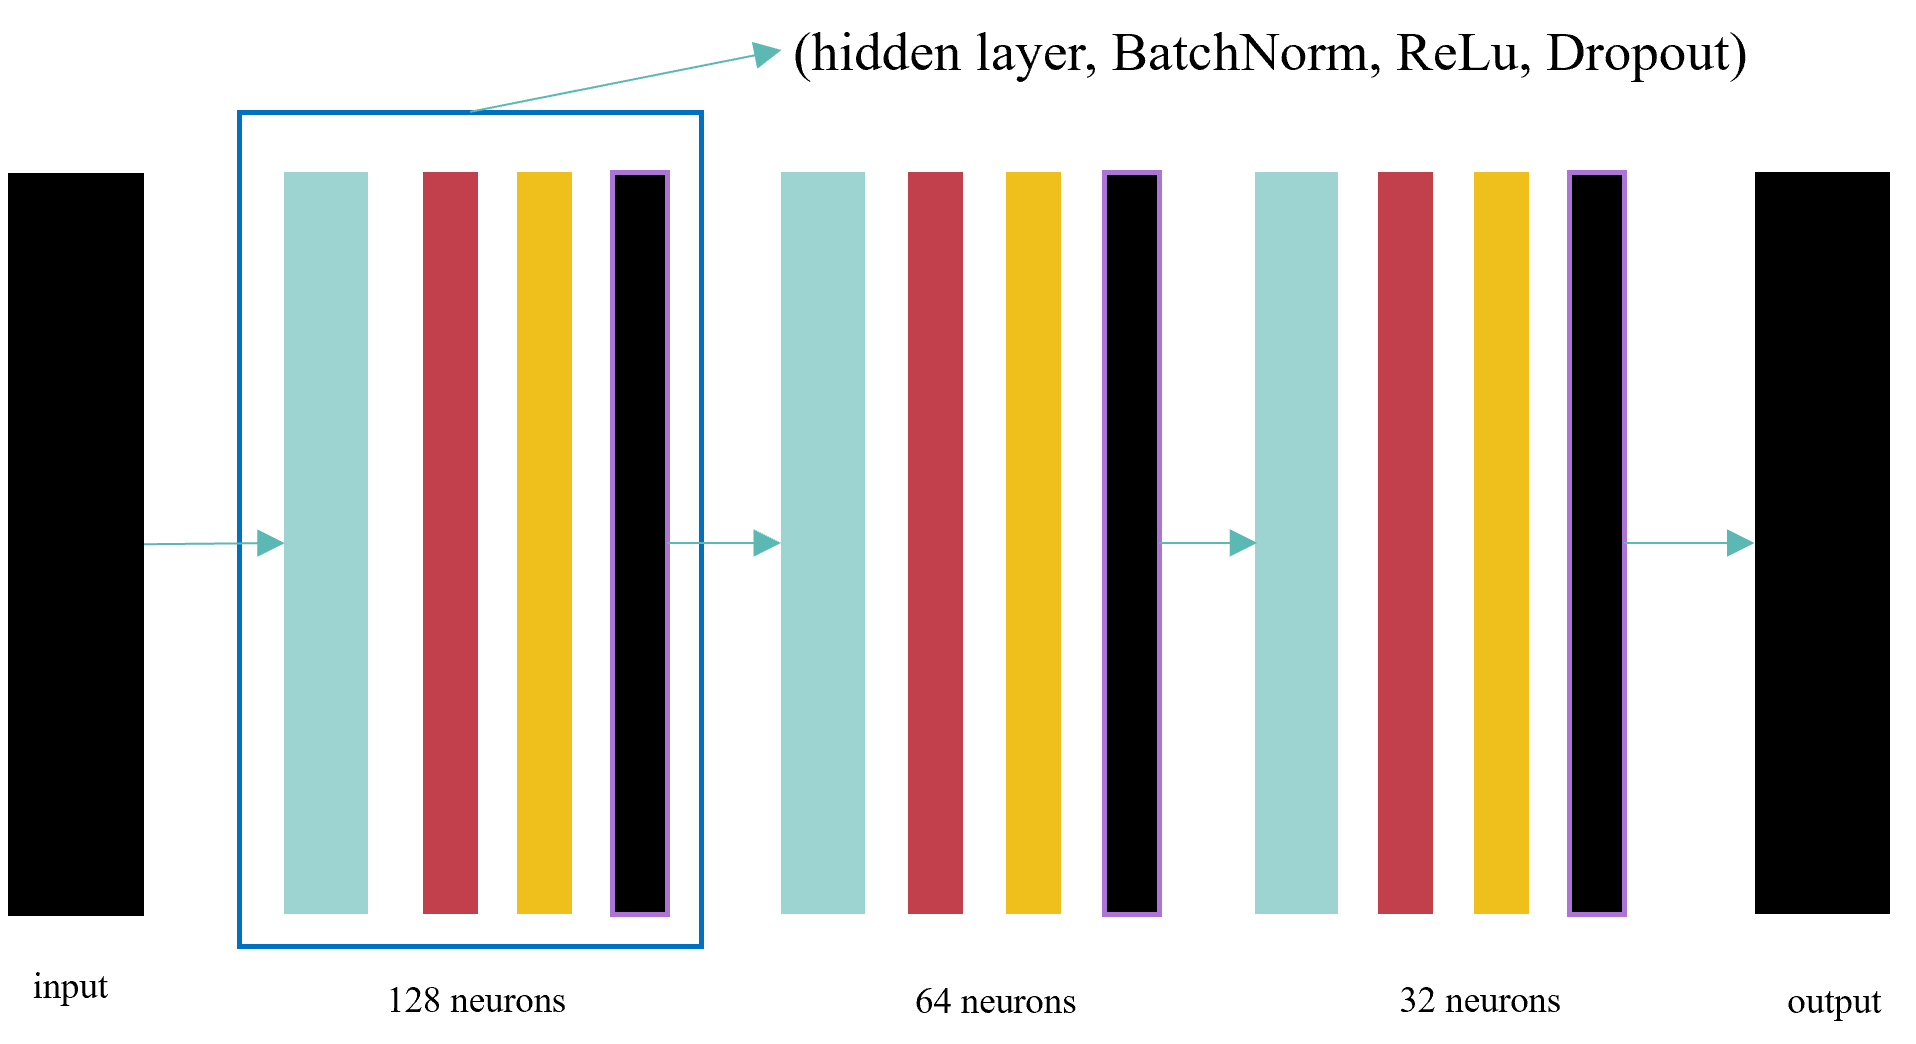
\includegraphics[width=0.9\textwidth]{images/architecture.png}
    \caption{Neural Network Architecture for Malware Detection}
    \label{fig:nn_architecture}
\end{figure}

The architecture is illustrated in Figure \ref{fig:nn_architecture}. The input layer accepts the processed feature set (the same as used by the traditional models), followed by three hidden layers with decreasing counts (128, 64, 32). The output layer uses a sigmoid activation function to produce a probability score for the binary classification task.

The neural network was implemented using PyTorch. The model was trained with a batch size of 128 and used the same train / validation / test split used for traditional machine learning models to ensure a fair comparison.

Before training machine learning models, we applied several preprocessing steps to ensure optimal performance, including feature scaling, categorical encoding, and class balancing. This was also done to ensure that the models could learn effectively from the data without being biased by irrelevant features or imbalanced classes. The following subsections detail these preprocessing steps.

\begin{enumerate}
    \item \textbf{Feature scaling}: Numerical features were standardised using z-score normalisation:
    \begin{equation}
        z_{i,j} = \frac{x_{i,j} - \mu_j}{\sigma_j}
    \end{equation}
    where $\mu_j$ and $\sigma_j$ are the mean and standard deviation of feature $j$ computed from the training set.
    
    \item \textbf{Categorical encoding}: Categorical features such as protocol and connection state were encoded using one-hot encoding:
    \begin{equation}
        \mathbf{x}^{\text{one-hot}}_{i,j} = 
        \begin{cases}
            1 & \text{if } x_{i,j} = \text{category}_k \\
            0 & \text{otherwise}
        \end{cases}
    \end{equation}
    For features with high cardinality, we used a threshold frequency of 0.01 to retain only significant categories.
    
    \item \textbf{Class balancing}: To address the moderate class imbalance, we applied the SMOTE to the training set. SMOTE generates synthetic examples in the feature space, for each minority class example $x_i$, by:
    \begin{equation}
        x_{\text{new}} = x_i + \lambda \cdot (x_{nn} - x_i)
    \end{equation}
    where $x_{nn}$ is one of the $k$-nearest neighbours of $x_i$ in the minority class, and $\lambda \in [0,1]$ is a random number.
\end{enumerate}

\subsubsection{Feature Selection}

Feature selection reduces model complexity and prevents overfitting by identifying the most informative features. We employed a multi-stage approach combining filter, wrapper, and embedded methods.

First, we applied correlation-based filtering to remove highly correlated features. For a pair of features $X_i$ and $X_j$ with a Pearson correlation coefficient $\rho_{ij}$ exceeding a threshold of 0.9, we remove the characteristic with a lower correlation to the target variable:

\begin{equation}
    \text{Remove } X_i \text{ if } |\rho_{ij}| > 0.9 \text{ and } |\rho_{iy}| < |\rho_{jy}|
\end{equation}

Next, we used Recursive Feature Elimination with Cross-Validation (RFECV) to identify the optimal feature subset. RFECV works by recursively eliminating features, starting from the full set of features, and removing the least important features based on a model's feature importance scores. At each iteration, the algorithm fits a model to the training data and computes a cross-validated score to determine the optimal number of features.

For tree-based models (Random Forest and XGBoost), we also leveraged their intrinsic feature importance metrics. For Random Forest, the importance of the feature $j$ is calculated as the total decrease in the impurity of the node weighted by the probability of reaching that node, averaged over all trees:

\begin{equation}
    \text{Importance}(X_j) = \frac{1}{B} \sum_{b=1}^{B} \sum_{t \in \mathcal{T}_b: v(t)=j} p(t) \cdot [\Delta i(t)]
\end{equation}

where $\mathcal{T}_b$ is the set of nodes in tree $b$, $v(t)$ is the variable used to split at node $t$, $p(t)$ is the probability of reaching node $t$, and $\Delta i(t)$ is the decrease in impurity at node $t$.

\subsection{Hyperparameter Optimisation}

To determine the optimal hyperparameters for each model, we used RandomizedSearchCV instead of the traditional grid search. This approach samples from hyperparameter distributions, allowing us to explore a broader parameter space more efficiently. The optimisation process minimised the negative F1 score by five-fold cross-validation:

\begin{equation}
    \theta^* = \underset{\theta \in \Theta}{\text{argmin}} \left\{ -\frac{1}{5} \sum_{k=1}^{5} \text{F1-score}(y_{val}^{(k)}, \hat{y}_{val}^{(k)}; \theta) \right\}
\end{equation}

where $\theta$ represents the hyperparameters, $\Theta$ is the hyperparameter space, and $(y_{val}^{(k)}, \hat{y}_{val}^{(k)})$ are the true and predicted labels for the $k$-th validation fold.

\begin{table}[h!]
    \centering
    \caption{Hyperparameter distributions used in RandomizedSearchCV}
    \label{tab:hyperparameter_ranges}
    \begin{tabular}{llp{5.5cm}}
    \hline
    \textbf{Algorithm} & \textbf{Hyperparameter} & \textbf{Distribution} \\
    \hline
    \multirow{7}{*}{Random Forest} & n\_estimators & randint(50, 300) \\
     & max\_depth & $\{$None, 5, 10, 15, 20, 25, 30, 35, 40, 45$\}$ \\
     & min\_samples\_split & randint(2, 20) \\
     & min\_samples\_leaf & randint(1, 10) \\
     & max\_features & $\{$'sqrt', 'log2', None$\}$ \\
     & bootstrap & $\{$True, False$\}$ \\
     & class\_weight & $\{$'balanced', 'balanced\_subsample', None$\}$ \\
    \hline
    \multirow{9}{*}{XGBoost} & n\_estimators & randint(50, 300) \\
     & max\_depth & randint(3, 10) \\
     & learning\_rate & uniform(0.01, 0.2) \\
     & subsample & uniform(0.7, 0.3) \\
     & colsample\_bytree & uniform(0.7, 0.3) \\
     & gamma & uniform(0, 0.5) \\
     & min\_child\_weight & randint(1, 6) \\
     & reg\_alpha & $\{0, 0.001, 0.01, 0.1, 1\}$ \\
     & reg\_lambda & $\{0, 0.001, 0.01, 0.1, 1\}$ \\
    \hline
    \end{tabular}
\end{table}
    
Note: randint(a, b) represents a discrete uniform distribution between integers a (inclusive) and b (exclusive), and uniform(a, b) represents a continuous uniform distribution where a is the location parameter and b is the scale parameter, resulting in a distribution between a and a+b.
\subsection{Model Evaluation Framework}

Our classification models were assessed using multiple metrics derived from the confusion matrix elements: True Positives ($TP$), True Negatives ($TN$), False Positives ($FP$) and False Negatives ($FN$). The following key metrics quantified different aspects of model performance:

\begin{equation}
\text{Accuracy} = \frac{TP + TN}{TP + TN + FP + FN}
\end{equation}

\begin{equation}
\text{Precision} = \frac{TP}{TP + FP}
\end{equation}

\begin{equation}
\text{Recall} = \frac{TP}{TP + FN}
\end{equation}

\begin{equation}
\text{F1-score} = 2 \times \frac{\text{Precision} \times \text{Recall}}{\text{Precision} + \text{Recall}}
\end{equation}

\begin{equation}
\text{False Positive Rate} = \frac{FP}{FP + TN}
\end{equation}

For threshold-independent assessment, we utilised the Area Under the Receiver Operating Characteristic (AUC-ROC) curve. For a classifier producing a score $s(x)$ for each instance, this metric is calculated as:

\begin{equation}
\text{AUC-ROC} = \frac{\sum_{i \in \mathcal{P}} \sum_{j \in \mathcal{N}} \mathbb{1}[s(x_i) > s(x_j)]}{|\mathcal{P}| \times |\mathcal{N}|}
\end{equation}

where $\mathcal{P}$ and $\mathcal{N}$ represent positive and negative example sets, and $\mathbb{1}[\cdot]$ is the indicator function.

In the security context, we prioritise false positive rates and recall, as missed attacks can compromise security, while excessive false alarms lead to alert fatigue. Detection latency was also measured to evaluate the viability of the real-time application.

The implementation of our framework followed these key steps:

\begin{enumerate}
    \item \textbf{Data partitioning}: Stratified sampling divided the dataset into training sets (70\%), validation (15\%), and test sets (15\%) while maintaining class distribution. This split was chosen to ensure sufficient data for training and validation while maintaining a separate test set for the final evaluation.
    
    \item \textbf{Cross-validation}: 5-fold stratified cross-validation was used during training to ensure robust performance estimation and mitigate overfit risk.
    
    \item \textbf{Hyperparameter optimisation}: The hyperparameters of the model were fine-tuned using the validation set, with the F1 score as the primary optimisation metric.
    
    \item \textbf{Test set evaluation}: The final assessment was conducted on the test set that remained unused during the training and hyperparameter tuning phases.
\end{enumerate}

The evaluation metrics were calculated for each model and the results were compared to identify the best-performing model for the malware detection task. The models were also evaluated on the basis of their computational efficiency, including training time and inference speed, to ensure practical applicability in real-world scenarios. The results of the evaluation are presented in the next section, where we discuss the performance of each model and their implications for the detection of IoT malware.